\documentclass[
	12pt,				% Tamanho da fonte
	openright,			% Capítulos começam em pág ímpar
	oneside,			% Para impressão em apenas um lado. Use 'twoside' para frente e verso
	a4paper,			% Tamanho do papel
	portuguese,			% Idioma adicional para hifenização
	brazil				% O idioma principal do documento
	]{abntex2}

% --- PACOTES BÁSICOS ---
\usepackage[utf8]{inputenc}		% Codificação do documento
\usepackage[T1]{fontenc}		% Seleção de códigos de fonte
\usepackage{indentfirst}		% Indenta o primeiro parágrafo de cada seção
\usepackage{color}				% Controle de cores
\usepackage{graphicx}			% Inclusão de gráficos
\usepackage{microtype} 			% Para melhorias na justificação
\usepackage{amsmath}  % Essencial para fórmulas matemáticas
\usepackage{amsfonts} % Para símbolos como o de conjuntos (R, N, Z)
\usepackage{amssymb}  % Símbolos extras
\graphicspath{{images/}}

% --- CONFIGURAÇÕES DE PACOTES ---
\usepackage[alf]{abntex2cite}	% Citações padrão ABNT (Autor-data)

% --- INFORMAÇÕES DO TCC ---
\titulo{Pseudo Aleatoriedade e Segurança Criptográfica: Uma Análise da Transição para Algoritmos Pós-Quânticos}
\autor{Jean Victor Borges de Abreu}
\local{Petrópolis - Rio de Janeiro}
\data{2026}
\orientador{Nome do Orientador}
\instituicao{FACULDADE DE EDUCAÇÃO TECNOLÓGICA DO ESTADO DO RIO DE JANEIRO FAETERJ/PETRÓPOLIS}
\preambulo{Trabalho de Conclusão de Curso apresentado à...}

% --- INÍCIO DO DOCUMENTO ---
\begin{document}

\imprimircapa
\imprimirfolhaderosto

\chapter{Resumo}

\chapter{Abstract}

\chapter{Lista de Figuras}

\chapter{Lista de Abreviaturas}

\boldmath FAETERJ: Faculdade de Educação Tecnológica do Estado do Rio de Janeiro 

% --- SUMÁRIO ---
\pdfbookmark[0]{\contentsname}{toc}
\tableofcontents*
\cleardoublepage
% --- ELEMENTOS TEXTUAIS ---
\textual
\chapter{Introdução}
A infraestrutura de segurança digital de grandes corporações, em sua maioria sustentada por ecossistemas como o Java, vivencia um momento de transição crítica. 
Visto que computadores operam sob lógica determinística e não podem gerar o 'acaso puro' sem fontes externas de entropia, a criptografia contemporânea torna-se dependente da robustez matemática dos Geradores de Números Pseudo Aleatórios (PRNGs). 

Durante décadas, bibliotecas de segurança confiaram em implementações consolidadas, como a classe java.security.SecureRandom, para garantir a integridade de chaves e certificados. 
Contudo, o setor presencia o ocaso da criptografia clássica: a padronização recente liderada pelo NIST indica que as fontes de entropia e os algoritmos de pseudo aleatoriedade tradicionais não são mais suficientes contra ataques baseados em vetores quânticos. 
Nesse cenário, se o gerador de números responsável pela criação de chaves for previsível para um sistema quântico, a estrutura de segurança da informação como um todo torna-se obsoleta. 

O presente artigo explora esse panorama de mudança, avaliando como a transição para a Criptografia Pós-Quântica (PQC) altera as práticas de desenvolvimento e investigando novos padrões de redes de pontos (lattices), 
bem como a adaptação da plataforma Java para assegurar a soberania dos dados em um futuro pós-quântico.
\section{Contextualização do Tema}

Com o avanço da tecnologia e o uso crescente de ferramentas e hardwares quanticos. 
A utilização de meios pesudoaleatorios tem sidos colocados em risco. 
E sua utilização em alguns anos podem se tornar obsoletos e inseguros para utilização. 
Como já é o caso de grandes empresas e organizações governamentais. 
Das quais já fazem uso de  outros meios para criptografar suas informações. 

\section{Justificativa/Problema de Pesquisa}

Muitos Textos

\section{Motivação/Hipotese e Ameaca Tecnológica}

Muitos textos

\section{Objetivos}

Muitos textos

\section{Metodologia}

Muitos textos

\chapter{FUNDAMENTOS DA ALEATORIEDADE EM COMPUTAÇÃO} % Capitulo 2

\section{Aleatoriedade Verdadeira vs. Pseudoaleatoriedade}

Muitos textos

\section{Entropia e Fontes de Incerteza}

Muitos textos

\section{A Semente (Seed) como Elemento Crítico}

Muitos textos

\section{Avaliação Estatística da Aleatoriedade}

Muitos textos

\chapter{Geradores Criptograficamente Seguros} % Capitulo 3

\section{RNGs vs. CSPRNGs}

Muitos textos

\section{O Ataque do Próximo Bit}

Muitos textos

\subsection{Implementação Prática (Demonstração)}

Muitos textos

\section{Implementação de CSPRNGs em Java}

Muitos textos

\section{Falhas Históricas de Aleatoriedade}

Muitos textos

\chapter{COMPUTAÇÃO QUÂNTICA E A QUEBRA DO PARADIGMA ATUAL} % Capitulo 4

\section{Conceitos Fundamentais de Computação Quântica}

Muitos textos

\section{Algoritmo de Shor}

Muitos textos

\section{Algoritmo de Grover}

Muitos textos

\section{Harvest Now, Decrypt Later}

Muitos textos

\chapter{CRIPTOGRAFIA PÓS-QUÂNTICA (PQC)} % Capitulo 5

\section{Definição e Objetivos da PQC}

Muitos textos

\section{Paradigmas Matemáticos da PQC}

Muitos textos

\section{Criptografia Baseada em Reticulados}

Muitos textos

\section{Learning With Errors (LWE)}

Muitos textos

\subsection{Implementação Didática em Java (Demonstração)}

Muitos textos

\section{Padronização Pós-Quântica}

Muitos textos

\chapter{A TRANSIÇÃO PARA PQC NO ECOSSISTEMA JAVA} % Capitulo 6

\section{Suporte à Criptografia Pós-Quântica no Java}

Muitos textos

\section{Crypto-Agility}

Muitos textos

\subsection{Implementação Prática: Demo de Crypto-Agility}

Muitos textos

\section{Comparativo de Modelos}

Muitos textos

\subsection{Implementação Prática: Benchmark Clássico vs. Kyber}

Muitos textos

\chapter{DISCUSSÃO E ANÁLISE CRÍTICA} % Capitulo 7

\section{Impacto em Desempenho}

Muitos textos

\section{Barreiras de Adoção}

Muitos textos

\section{Implicações Sociais e Éticas}

Muitos textos

\chapter{DISCUSSÃO E ANÁLISE CRÍTICA} % Capitulo 8 - Conclusao

\section{Síntese dos Resultados}

Muitos textos

\section{Resposta ao Problema de Pesquisa}

Muitos textos

\section{Trabalhos Futuros}

Muitos textos

\chapter{Coisas possivelmente Uteis em algum momento}

PRNG é uma sigla para “Pseudo Random Number Generator” ou “Gerador de Números Pseudo Aleatórios”. 
Seu significado é que a sua geração de números não segue uma estrutura aleatória. 
Ele utiliza um ponto inicial denominado “seed” para dar início a sua geração de números. 
A seed é um valor base para ser utilizado no PRNG. 
Utilizando a mesma seed, o resultado final do PRNG será o mesmo.

O PRNG funciona a partir de uma função que recebe a seed por parâmetro. 
E através de um cálculo, ele retorna o resultado dessa fórmula. 
Uma das fórmulas mais comuns para esse tipo de gerador de pseudo números aleatórios é no modelo LCG “Gerador Congruencial Linear” 

\begin{equation}
    x_{i+1} = (A \cdot x_i + C) \pmod{M}
    \label{eq:lca}
\end{equation}

Onde o valor inicial “x0” é a seed, A e C são parâmetros inteiros que podem ter um valor já pré-definido ou passados diretamente, M é o espaço dos valores aleatórios possíveis e “mod” é o restante da divisão inteira.


\begin{figure}[htb]
    \centering
    \caption{Modelo simples de um PRNG com LCG}
    \label{fig:model_prng_lcg}
    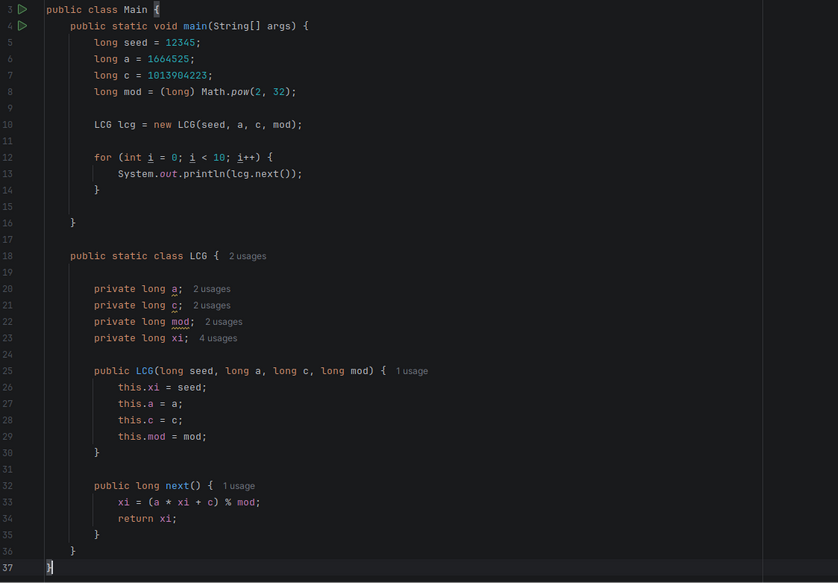
\includegraphics[width=0.8\textwidth]{model_prng_lcg.png}
    \legend{Fonte: Elaborado pelo autor (2026)}
\end{figure}

Mesmo após inúmeras tentativas. Devido a seed permanecer inalterada. 
O resultado permanece o mesmo em todos os resultados obtidos.

Por mais que tenha se passado um valor fixo na seed no exemplo prático, a seed é definida pelo sistema operacional, esse número é denominado entropia. 
Que se tem por referência a quantidade de imprecisão de um sistema. 
Quanto maior o número da entropia, maior é a incerteza. 
Esse valor de entropia é gerado a partir de certos eventos que ocorrem no momento de sua captura, como por exemplo o movimento do mouse, os inputs no teclado etc. 
Essas capturas são convertidas em um valor numérico para ser usado na seed.

Esses inputs que o sistema captura podem ser previsíveis, tornando a entropia causada menor. 
Sendo possível pré-determinar o valor gerado ao final para seed. 
Apesar das aplicações para o dia a dia ou em pequenos projetos serem o suficiente. 
Esse método  não é seguro para aplicações de alto risco.


\begin{figure}[htb]
    \centering
    \caption{Resultado do script LCG}
    \label{fig:result_prng_lcg}
    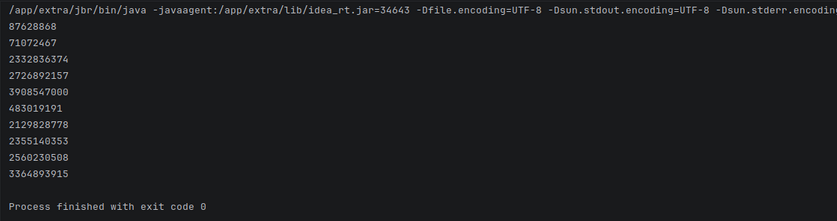
\includegraphics[width=0.8\textwidth]{result_prng_lcg.png}
    \legend{Fonte: Elaborado pelo autor (2026)}
\end{figure}

\chapter{Conclusão}
Considerações finais.

% --- ELEMENTOS PÓS-TEXTUAIS ---
\postextual
\bibliography{referencias} % Arquivo .bib com suas fontes

\end{document}